% This file was created with tikzplotlib v0.10.1.
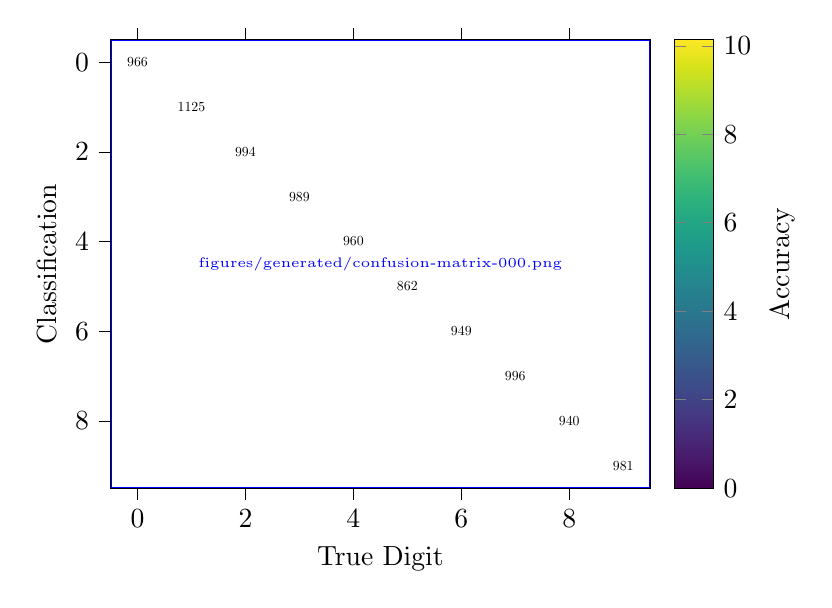
\begin{tikzpicture}

  \definecolor{darkgray176}{RGB}{176,176,176}

  \begin{axis}[
      colorbar,
      colorbar style={ylabel={Accuracy}},
      colormap/viridis,
      point meta max=10.1369911120802,
      point meta min=0,
      tick align=outside,
      x grid style={darkgray176},
      xlabel={True Digit},
      xmin=-0.5, xmax=9.5,
      xtick pos=both,
      xtick style={color=black},
      y dir=reverse,
      y grid style={darkgray176},
      ylabel={Classification},
      ymin=-0.5, ymax=9.5,
      ytick pos=left,
      ytick style={color=black}
    ]
    \addplot graphics [includegraphics cmd=\pgfimage,xmin=-0.5, xmax=9.5, ymin=9.5, ymax=-0.5] {figures/generated/confusion-matrix-000.png};
    \draw (axis cs:0,0) node[
      scale=0.5,
      text=black,
      rotate=0.0
    ]{966};
    \draw (axis cs:1,0) node[
      scale=0.5,
      text=white,
      rotate=0.0
    ]{0};
    \draw (axis cs:2,0) node[
      scale=0.5,
      text=white,
      rotate=0.0
    ]{2};
    \draw (axis cs:3,0) node[
      scale=0.5,
      text=white,
      rotate=0.0
    ]{0};
    \draw (axis cs:4,0) node[
      scale=0.5,
      text=white,
      rotate=0.0
    ]{1};
    \draw (axis cs:5,0) node[
      scale=0.5,
      text=white,
      rotate=0.0
    ]{1};
    \draw (axis cs:6,0) node[
      scale=0.5,
      text=white,
      rotate=0.0
    ]{4};
    \draw (axis cs:7,0) node[
      scale=0.5,
      text=white,
      rotate=0.0
    ]{3};
    \draw (axis cs:8,0) node[
      scale=0.5,
      text=white,
      rotate=0.0
    ]{2};
    \draw (axis cs:9,0) node[
      scale=0.5,
      text=white,
      rotate=0.0
    ]{1};
    \draw (axis cs:0,1) node[
      scale=0.5,
      text=white,
      rotate=0.0
    ]{0};
    \draw (axis cs:1,1) node[
      scale=0.5,
      text=black,
      rotate=0.0
    ]{1125};
    \draw (axis cs:2,1) node[
      scale=0.5,
      text=white,
      rotate=0.0
    ]{3};
    \draw (axis cs:3,1) node[
      scale=0.5,
      text=white,
      rotate=0.0
    ]{0};
    \draw (axis cs:4,1) node[
      scale=0.5,
      text=white,
      rotate=0.0
    ]{0};
    \draw (axis cs:5,1) node[
      scale=0.5,
      text=white,
      rotate=0.0
    ]{1};
    \draw (axis cs:6,1) node[
      scale=0.5,
      text=white,
      rotate=0.0
    ]{3};
    \draw (axis cs:7,1) node[
      scale=0.5,
      text=white,
      rotate=0.0
    ]{1};
    \draw (axis cs:8,1) node[
      scale=0.5,
      text=white,
      rotate=0.0
    ]{2};
    \draw (axis cs:9,1) node[
      scale=0.5,
      text=white,
      rotate=0.0
    ]{0};
    \draw (axis cs:0,2) node[
      scale=0.5,
      text=white,
      rotate=0.0
    ]{5};
    \draw (axis cs:1,2) node[
      scale=0.5,
      text=white,
      rotate=0.0
    ]{1};
    \draw (axis cs:2,2) node[
      scale=0.5,
      text=black,
      rotate=0.0
    ]{994};
    \draw (axis cs:3,2) node[
      scale=0.5,
      text=white,
      rotate=0.0
    ]{7};
    \draw (axis cs:4,2) node[
      scale=0.5,
      text=white,
      rotate=0.0
    ]{1};
    \draw (axis cs:5,2) node[
      scale=0.5,
      text=white,
      rotate=0.0
    ]{0};
    \draw (axis cs:6,2) node[
      scale=0.5,
      text=white,
      rotate=0.0
    ]{3};
    \draw (axis cs:7,2) node[
      scale=0.5,
      text=white,
      rotate=0.0
    ]{10};
    \draw (axis cs:8,2) node[
      scale=0.5,
      text=white,
      rotate=0.0
    ]{8};
    \draw (axis cs:9,2) node[
      scale=0.5,
      text=white,
      rotate=0.0
    ]{3};
    \draw (axis cs:0,3) node[
      scale=0.5,
      text=white,
      rotate=0.0
    ]{0};
    \draw (axis cs:1,3) node[
      scale=0.5,
      text=white,
      rotate=0.0
    ]{0};
    \draw (axis cs:2,3) node[
      scale=0.5,
      text=white,
      rotate=0.0
    ]{1};
    \draw (axis cs:3,3) node[
      scale=0.5,
      text=black,
      rotate=0.0
    ]{989};
    \draw (axis cs:4,3) node[
      scale=0.5,
      text=white,
      rotate=0.0
    ]{1};
    \draw (axis cs:5,3) node[
      scale=0.5,
      text=white,
      rotate=0.0
    ]{5};
    \draw (axis cs:6,3) node[
      scale=0.5,
      text=white,
      rotate=0.0
    ]{0};
    \draw (axis cs:7,3) node[
      scale=0.5,
      text=white,
      rotate=0.0
    ]{4};
    \draw (axis cs:8,3) node[
      scale=0.5,
      text=white,
      rotate=0.0
    ]{2};
    \draw (axis cs:9,3) node[
      scale=0.5,
      text=white,
      rotate=0.0
    ]{8};
    \draw (axis cs:0,4) node[
      scale=0.5,
      text=white,
      rotate=0.0
    ]{0};
    \draw (axis cs:1,4) node[
      scale=0.5,
      text=white,
      rotate=0.0
    ]{0};
    \draw (axis cs:2,4) node[
      scale=0.5,
      text=white,
      rotate=0.0
    ]{2};
    \draw (axis cs:3,4) node[
      scale=0.5,
      text=white,
      rotate=0.0
    ]{1};
    \draw (axis cs:4,4) node[
      scale=0.5,
      text=black,
      rotate=0.0
    ]{960};
    \draw (axis cs:5,4) node[
      scale=0.5,
      text=white,
      rotate=0.0
    ]{0};
    \draw (axis cs:6,4) node[
      scale=0.5,
      text=white,
      rotate=0.0
    ]{7};
    \draw (axis cs:7,4) node[
      scale=0.5,
      text=white,
      rotate=0.0
    ]{2};
    \draw (axis cs:8,4) node[
      scale=0.5,
      text=white,
      rotate=0.0
    ]{1};
    \draw (axis cs:9,4) node[
      scale=0.5,
      text=white,
      rotate=0.0
    ]{9};
    \draw (axis cs:0,5) node[
      scale=0.5,
      text=white,
      rotate=0.0
    ]{2};
    \draw (axis cs:1,5) node[
      scale=0.5,
      text=white,
      rotate=0.0
    ]{0};
    \draw (axis cs:2,5) node[
      scale=0.5,
      text=white,
      rotate=0.0
    ]{0};
    \draw (axis cs:3,5) node[
      scale=0.5,
      text=white,
      rotate=0.0
    ]{10};
    \draw (axis cs:4,5) node[
      scale=0.5,
      text=white,
      rotate=0.0
    ]{2};
    \draw (axis cs:5,5) node[
      scale=0.5,
      text=black,
      rotate=0.0
    ]{862};
    \draw (axis cs:6,5) node[
      scale=0.5,
      text=white,
      rotate=0.0
    ]{8};
    \draw (axis cs:7,5) node[
      scale=0.5,
      text=white,
      rotate=0.0
    ]{0};
    \draw (axis cs:8,5) node[
      scale=0.5,
      text=white,
      rotate=0.0
    ]{5};
    \draw (axis cs:9,5) node[
      scale=0.5,
      text=white,
      rotate=0.0
    ]{3};
    \draw (axis cs:0,6) node[
      scale=0.5,
      text=white,
      rotate=0.0
    ]{1};
    \draw (axis cs:1,6) node[
      scale=0.5,
      text=white,
      rotate=0.0
    ]{1};
    \draw (axis cs:2,6) node[
      scale=0.5,
      text=white,
      rotate=0.0
    ]{0};
    \draw (axis cs:3,6) node[
      scale=0.5,
      text=white,
      rotate=0.0
    ]{1};
    \draw (axis cs:4,6) node[
      scale=0.5,
      text=white,
      rotate=0.0
    ]{3};
    \draw (axis cs:5,6) node[
      scale=0.5,
      text=white,
      rotate=0.0
    ]{2};
    \draw (axis cs:6,6) node[
      scale=0.5,
      text=black,
      rotate=0.0
    ]{949};
    \draw (axis cs:7,6) node[
      scale=0.5,
      text=white,
      rotate=0.0
    ]{0};
    \draw (axis cs:8,6) node[
      scale=0.5,
      text=white,
      rotate=0.0
    ]{1};
    \draw (axis cs:9,6) node[
      scale=0.5,
      text=white,
      rotate=0.0
    ]{0};
    \draw (axis cs:0,7) node[
      scale=0.5,
      text=white,
      rotate=0.0
    ]{1};
    \draw (axis cs:1,7) node[
      scale=0.5,
      text=white,
      rotate=0.0
    ]{6};
    \draw (axis cs:2,7) node[
      scale=0.5,
      text=white,
      rotate=0.0
    ]{9};
    \draw (axis cs:3,7) node[
      scale=0.5,
      text=white,
      rotate=0.0
    ]{3};
    \draw (axis cs:4,7) node[
      scale=0.5,
      text=white,
      rotate=0.0
    ]{2};
    \draw (axis cs:5,7) node[
      scale=0.5,
      text=white,
      rotate=0.0
    ]{0};
    \draw (axis cs:6,7) node[
      scale=0.5,
      text=white,
      rotate=0.0
    ]{0};
    \draw (axis cs:7,7) node[
      scale=0.5,
      text=black,
      rotate=0.0
    ]{996};
    \draw (axis cs:8,7) node[
      scale=0.5,
      text=white,
      rotate=0.0
    ]{2};
    \draw (axis cs:9,7) node[
      scale=0.5,
      text=white,
      rotate=0.0
    ]{9};
    \draw (axis cs:0,8) node[
      scale=0.5,
      text=white,
      rotate=0.0
    ]{4};
    \draw (axis cs:1,8) node[
      scale=0.5,
      text=white,
      rotate=0.0
    ]{0};
    \draw (axis cs:2,8) node[
      scale=0.5,
      text=white,
      rotate=0.0
    ]{1};
    \draw (axis cs:3,8) node[
      scale=0.5,
      text=white,
      rotate=0.0
    ]{6};
    \draw (axis cs:4,8) node[
      scale=0.5,
      text=white,
      rotate=0.0
    ]{5};
    \draw (axis cs:5,8) node[
      scale=0.5,
      text=white,
      rotate=0.0
    ]{3};
    \draw (axis cs:6,8) node[
      scale=0.5,
      text=white,
      rotate=0.0
    ]{7};
    \draw (axis cs:7,8) node[
      scale=0.5,
      text=white,
      rotate=0.0
    ]{3};
    \draw (axis cs:8,8) node[
      scale=0.5,
      text=black,
      rotate=0.0
    ]{940};
    \draw (axis cs:9,8) node[
      scale=0.5,
      text=white,
      rotate=0.0
    ]{5};
    \draw (axis cs:0,9) node[
      scale=0.5,
      text=white,
      rotate=0.0
    ]{2};
    \draw (axis cs:1,9) node[
      scale=0.5,
      text=white,
      rotate=0.0
    ]{2};
    \draw (axis cs:2,9) node[
      scale=0.5,
      text=white,
      rotate=0.0
    ]{0};
    \draw (axis cs:3,9) node[
      scale=0.5,
      text=white,
      rotate=0.0
    ]{3};
    \draw (axis cs:4,9) node[
      scale=0.5,
      text=white,
      rotate=0.0
    ]{10};
    \draw (axis cs:5,9) node[
      scale=0.5,
      text=white,
      rotate=0.0
    ]{3};
    \draw (axis cs:6,9) node[
      scale=0.5,
      text=white,
      rotate=0.0
    ]{1};
    \draw (axis cs:7,9) node[
      scale=0.5,
      text=white,
      rotate=0.0
    ]{5};
    \draw (axis cs:8,9) node[
      scale=0.5,
      text=white,
      rotate=0.0
    ]{2};
    \draw (axis cs:9,9) node[
      scale=0.5,
      text=black,
      rotate=0.0
    ]{981};
  \end{axis}

\end{tikzpicture}
